\documentclass[12pt]{article}
\usepackage{amsmath}
\usepackage{amssymb}
\usepackage{geometry}
\usepackage{enumerate}
\usepackage{natbib}
\usepackage{float}%稳定图片位置
\usepackage{graphicx}%画图
\usepackage[english]{babel}
\usepackage{a4wide}
\usepackage{indentfirst}%缩进
\usepackage{enumerate}%加序号
\usepackage{multirow}%合并行
\title{\large UM-SJTU JOINT INSTITUTE\\PHYSICS LABTORATORY\\(VE216)\\\ \\\ \\\ \\\ \\\ \\\ \\\ \\\ \\\ \\\ \\\
LABTORATORY REPORT\\\ \\\ LAB 2\\\ AM RADIO \\\ \\\ \\\ \\\ \\\ }
\author{Name: Pan Chongdan\\ID: 516370910121\\Name Xiang Zhiyuan\\ID: 516370910126}
\date{Date: \today}

\begin{document}
\maketitle
\newpage
\section{Objectives}
\begin{itemize}
\item Understand the principle of envelope detector and its relationship with Amplitude Modulation
\item Review op amp circuits
\item Learn about resonance phenomena and simple RLC bandpass filters
\item Learn a bit about antennas.
\item Learn basic superheterodyne receiver operating principles, since theses principles play a critical role in
many radio and signal processing systems.
\item Use the frequency domain concepts learned in your EECS 216 lectures to analyze the operation of a
superheterodyne AM radio receiver. Learn about mixing and its effect on the signal spectrum. Observe
the demodulation of an AM signal using an envelope detector.
\item Construct a fully operational superheterodyne AM radio and demonstrate that it operates as predicted
by theory.
\item Gain an appreciation of the fact that the mathematical tools you are learning in EECS 216 can be
used to design and build interesting and useful systems.
\end{itemize}
\section{Theoretical Background}
Fundamentally, AM modulation and demodulation are based on the Fourier transform modulation property.
\begin{equation}
s(t)\cos(\omega_{LO}t)\leftrightarrow\frac{1}{2}S(j(\omega-\omega_{LO}))+\frac{1}{2}S(j(\omega+\omega_{LO}))
\end{equation}
The actual translation of this mathematical fact into a practical electrical system of a functioning
radio is discussed here. The development is rather long and covers the design of a radio from the antenna
all the way to the last stage of demodulation.
\subsection{Transmitted Signal}
The transmitted AM (amplitude modulated) signal is of the form $x(t)=(A+bs(t))\cos(\omega_ct+\phi)$In Lab
2, you observed signals $x(t)$ of this form with $s(t)$ a sinusoid or a triangular wave. The carrier is specified
by $\cos(\omega_ct+\phi),f_c=\frac{\omega_c}{2\pi}$ is the carrier frequency in Hz, $s(t)$ is the “information or message” that is beingsent, e.g., voice, data, or music, and $A$ and $b$ are constants. The constants $A$ and $b$ are chosen to ensure
the condition $A+bs(t)\ge0$, which, from Lab 2, you know to be important for envelope detection. The
modulation depth, specified as a percentage, is defined as
\begin{equation}
\frac{\text{msx}(bs(t))-\text{min}(bs(t))}{2A}\times 100\%
\end{equation}
\par In commercial broadcast AM, the US Federal Communications Commission (FCC) specifies that the
carrier frequency must be one of the following 117 values
\begin{equation}
f_c=540KHz+(i-1)\times 10KHz,i=1,2,\cdots,117
\end{equation}
and thus spans a range from 540 KHz to 1700 KHz in increments of 10 KHz. The carrier frequencies given
by this formula correspond to the frequencies on your radio dial (AM).
\begin{figure}[H]
\centering
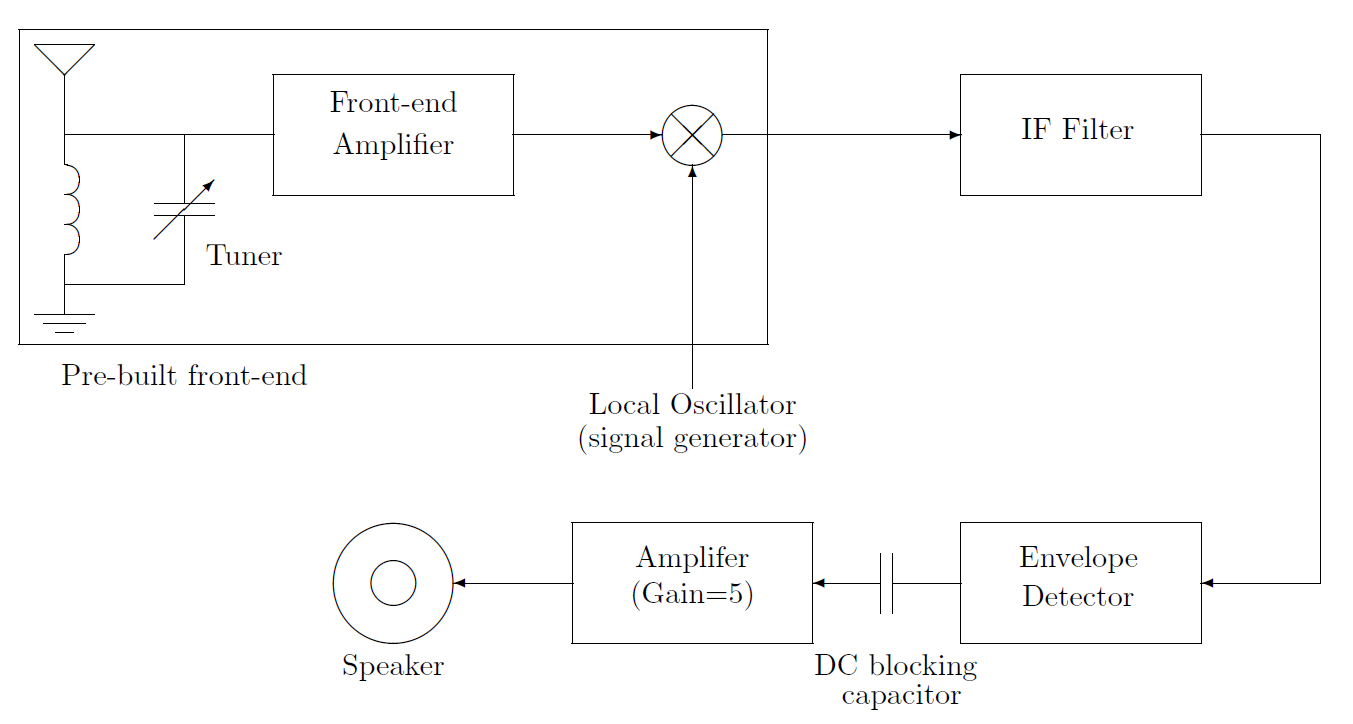
\includegraphics[scale=0.3]{P1.jpg}
\caption{AM Superheterodyne Radio Block Diagram}
\end{figure}
The information signal itself, $s(t)$, is a baseband signal with a bandwidth of 5 KHz, i.e., $|S(j\omega)|\approx0$ for
$\omega>2\pi\cdot 5000 \text{rad/s}$, where $S(j\omega)$ is the Fourier transform of a long segment of the signal (music, data or voice), $s(t)$. Thus the information signal contains little power at frequencies beyond 5 KHz. Younger adults
can hear frequencies up to nearly 20 KHz, and thus commercial AM broadcasts do not transmit music with
high fidelity, even in the absence of noise. This is not a limitation imposed by the method of amplitude
modulation per se, but rather a consequence of the narrow bandwidth assigned by the FCC when broadcast
AM radio was created. We could change this at any time if we were willing to absorb the huge cost of
replacing the thousands of transmitters and millions of receivers in existence today.
\subsection{Pre-built Front-end: Antenna \& Tuned RLC Circuit}
The “front-end” of the radio you will use in the lab has been pre-built and packaged for you. It consists
of a tuned RLC circuit, a field effect transistor (FET) pre-amplifier and a mixer. The tuned RLC circuit,
in addition to providing some filtering, also serves as an antenna. The antenna/tuned RLC circuit can be
modeled by the circuit shown in Fig. 2 below.
\begin{figure}[H]
\centering
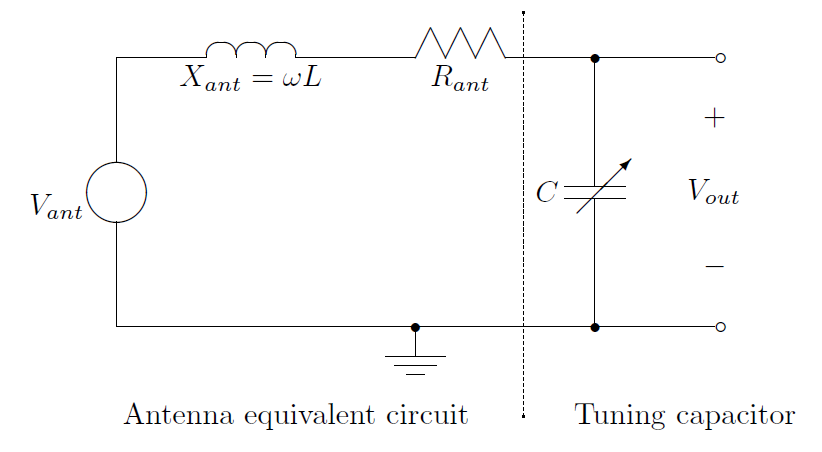
\includegraphics[scale=0.5]{P2.jpg}
\caption{Antenna/Front-end Tuned RLC Circuit (preamplifier and mixer not shown)}
\end{figure}
\par As will be described later, the inductor value is fixed at approximately 960 $\mu H$, the antenna resistance
$R_{ant}$ is frequency dependent, increasing with frequency, and C is a user-controllable variable capacitor. It
is a straightforward exercise to compute $\frac{V_{out}(j\omega)}{V_{ant}(j\omega)}$ as a function of frequency $\omega$. It will be assumed that the output of the circuit is connected to a very high impedance input (e.g., the input of a field effect transistor (FET)), and thus is essentially open-circuited. The quantity 20 log$\frac{V_{out}(j\omega)}{V_{ant}(j\omega)}$
dB has been computed and is
plotted in Fig. 3 for two different RLC combinations, i.e., $R_{ant}=200\Omega, L=960\mu H, C = 15 pF$ and
$R_{ant}=50\Omega, L=960\mu H, C = 75 pF$. Note that this circuit acts as a bandpass filter whose center frequency is determined by the value of the capacitor, which is tunable by the radio listener. The capacitor value is
chosen by the listener so that the center frequency of the bandpass filter corresponds to the carrier frequency
of the desired AM station.
\begin{figure}[H]
\centering
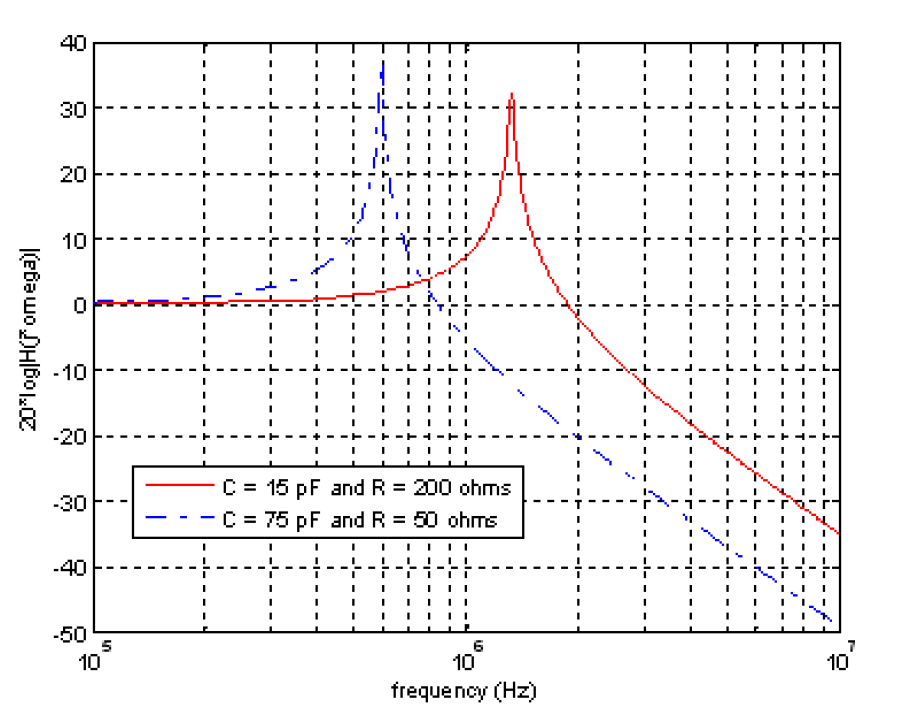
\includegraphics[scale=0.5]{P3.jpg}
\caption{Frequency Response of Tuned RLC Front-End}
\end{figure}
\subsubsection{Antenna (or How to Efficiently Receive a Signal)}
Antennas can take many different forms depending on the application. In your radio, the receiving
antenna is a coil of wire wound around a ferrite core, i.e., an electrically non-conducting material with
special magnetic properties. Such a coil depicted in Fig. 4(a) is known as a “loopstick” and is commonly
used for the antenna in AM radios.
\begin{figure}[H]
\centering
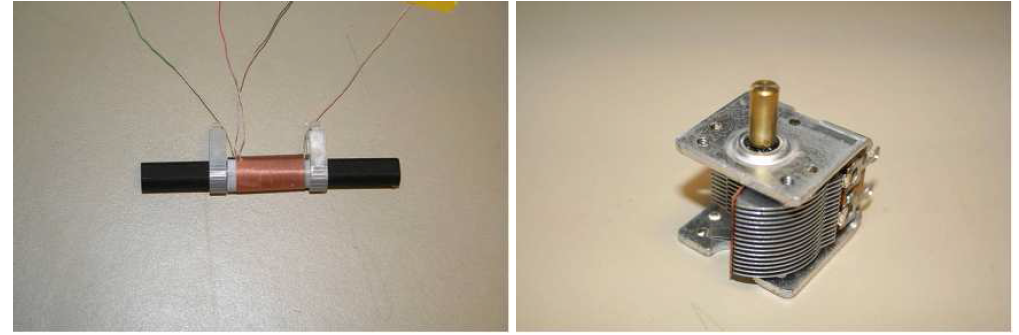
\includegraphics[scale=0.5]{P4.jpg}
\caption{(a) A Loopstick Antenna (b) Variable Capacitor}
\end{figure}
\par The carrier wavelength,$\lambda_c$, is given by $\lambda_c=\frac{c}{f_c}$, where c is the vacuum speed of light, $3x10^8$ m/s, and $f_c$ is the carrier frequency in Hz, which for commercial AM lies between 540 KHz and 1700 KHz. Thus the
carrier wavelength is on the order of a few hundred meters. The electrical properties of an antenna can be
modeled by a Thevenin equivalent circuit consisting of a voltage source, $V_{ant}$, in series with an impedance,
$Z_{ant}=R_{ant} + jX_{ant}$ as shown in Fig. 5.
\begin{figure}[H]
\centering
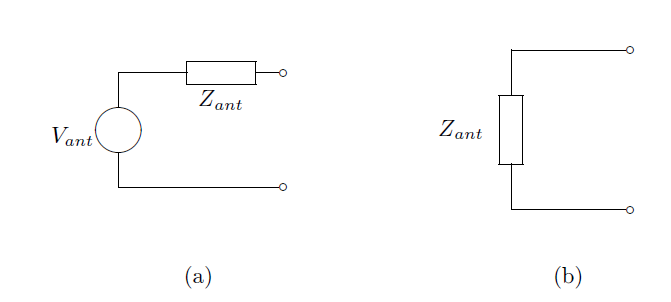
\includegraphics[scale=0.5]{P5.jpg}
\caption{Thevenin Equivalent Circuit Model for an Antenna (a) Receiving, (b) Transmitting;}
\end{figure}
\par $Z_{ant}$ is the same whether the antenna is transmitting or receiving a signal. $V_{ant}$, on the other hand, is only
non-zero when the antenna is receiving a signal. Time-varying electric and magnetic fields are associated with
the transmission of radio waves. According to Faraday’s Law of electromagnetics, a time-varying magnetic
field radiated from a distant transmitter will induce an (open-loop) voltage drop, $V_{ant}$, across the ends of
the coil in a loopstick receiving antenna (in particular, the voltage induced across the ends of a loop of
wire equals the rate of change of flux through that loop). The voltage drop will be proportional to the
product of the square-root of the power of the transmitted radio wave measured at the receiving antenna,
the cross-sectional area of the coil, the number of turns in the coil and the relative permeability of the ferrite
core.
\par $R_{ant}$ is the sum of three resistive terms (1) the radiation resistance $R_r$ of the antenna, (2) the resistance
$R_{coil}$ of the coil wire and (3) the magnetic losses (due to hysteresis) in the core $R_{core}$,
\begin{equation}
R_{ant}=R_r+R_{coil}+R_{core}
\end{equation}
The coil wire and the core magnetic losses are parasitic effects, and with ideal materials (i.e., perfectly
conducting coil wires and ferrites without hysteresis), these resistive terms would be zero. The radiation resistance, as the name implies, is associated with the radiation and reception of electromagnetic radiation
(i.e., radio waves) and is not actually a loss term. If a sinusoidal voltage source is applied across the ends
of the antenna coil when used as a transmitting antenna, a current will flow in the coil. The ratio of the
applied voltage to current, assuming that $R_{coil}$ and $R_{core}$ are zero, is given by the radiation resistance.
Furthermore the time-averaged power radiated away from the antenna in the form of an electromagnetic
wave is given by the product of 1/2 the square of the current and the radiation resistance (i.e., the power that
would be dissipated by a real resistor of $R_{ant}\Omega$). Similarly when operated as a receiving antenna, the
current flowing through an attached load of impedance $Z_L$ will be given by $I_L= \frac{V_ant}{(Z_{ant}+Z_L)}$. This current
not only delivers signal power to the load but also drives the antenna to re-radiate some of the received
electromagnetic signal. The time-averaged power that is re-radiated is given by the product of 1/2 the square
of the current and the radiation resistance.
\par The radiation resistance of a loopstick receiving antenna is negligible ($\ll 1\Omega$) when the size of the
antenna is small relative to a wavelength (as it is in our case) and can be ignored. The coil and ferrite core
resistance values increase with frequency, but together remain below a few hundred ohms at commercial
AM carrier frequencies. The reactance of the antenna is inductive and corresponds to an inductor value of
approximately 960 $\mu H$ for our loopstick. The use of a ferrite core, as opposed to a hollow air core, greatly
increases (by a factor of several hundred to a thousand) the strength of the magnetic field inside the coil, and
hence the Thevenin equivalent voltage, $V_{ant}$. It also increases the inductance by an identical multiplicative
factor.
\par In general, why should one care about the impedance of an antenna? Well suppose that the antenna is
being used for transmission. The output of the transmitter, which generates some voltage, is applied across
the antenna terminals. The transmitter output can be modeled as Thevein equivalent voltage, $V_{trans}$, in series with a Thevenin equivalent impedance, $Z_{trans}$. The power radiated by the antenna will then be given by
\begin{equation}
P_{rad}=\frac{1}{2}|\frac{V_{trans}}{Z_{ant}+Z_{trans}}|^2R_{ant}
\end{equation}
This power will be a maximum when the transmitter is designed to yield $R_{trans}\approx0$ and $X_{trans}=-X_{ant}$,
yielding
\begin{equation}
\text{max}(P_{rad})=\frac{1}{2}|\frac{V_{trans}}{R_r+R_{coil}+R_{core}}|^2R_{r}^2
\end{equation}
Thus the fraction of the power radiated by the antenna (as opposed to being dissipated “needlessly” in the
coil and core) is given by
$$(\frac{R_r}{R_r+R_{coil}+R_{core}})$$
\par Clearly the efficiency increases as the size of $R_{coil}+R_{core}$ can be reduced relative to the radiation resistance.
Unfortunately, antennas that are small relative to the wavelength of the signal being transmitted generally
have very small radiation resistances and thus are inefficient radiators.
\par A similar analysis can be performed when the antenna is used for reception rather than transmission.
The received power dissipated in $R_{coil}+R_{core}$ is wasted. Furthermore, the issue of noise becomes important.
The ability to communicate with high fidelity is ultimately limited by the presence of noise/interference.
Some noise is present in the atmosphere, for example that due to lightning strikes around the world, while
some is produced by the electronics themselves inside the radio. It is a fundamental fact of physics that it is impossible to completely remove the electronics noise because it is due to the thermal agitation of electrons
in the circuit elements. In situations where the external atmospheric noise is negligible in comparison to
the signal level and the signal level is very weak, it is important to deliver as much of the received signal as
possible to the load in order to overcome the noise due to the radio electronics. We know that maximum
power delivery from the antenna to the load occurs when the impedance of the load is matched to that of
the antenna. Let us assume for the moment that we have an antenna with very low parasitic resistance,
$R_{coil}+R_{core}$, which is good from an efficiency point of view. In order to deliver maximum power from
the antenna to the load under such conditions, the front-end receiver electronics must be designed to be
impedance matched, i.e., $Z_{load}=Z^{*}_{ant}$. For small (relative to the wavelength) antennas, however, this is
very difficult to achieve because Rr is very small.
\par In the AM radio band, atmospheric noise and interference are generally much larger than the electronics
noise. Thus the fidelity is not limited by the electronics noise and therefore impedance matching of the load
to the antenna is not critical as long as a reasonable signal level is provided to the load.
\subsubsection{RLC Resonant Circuit (or the First Step in Selecting a Station)}
The variable capacitor indicated in Fig. 2 consists of two sets of interleaved parallel metallic plates as
shown in Fig. 4(b). One set of the plates can be rotated relative to the other, thus varying the overlap
between the two plate sets, which in turn causes the capacitance to change. The capacitance ranges from
about 10 pF when there is no overlap between the plates to 400 pF when the plates are fully overlapped.
\par The loopstick antenna together with the capacitor shown in Fig. 2 is a series RLC resonance circuit.
Since this type of circuit and resonance phenomena in general play such an important role in electrical
engineering, we will digress briefly to discuss these topics in some further detail below.
\par The current flowing in the RLC circuit will be a maximum when the series RLC impedance is minimum.
This impedance minimum occurs at a frequency for which the reactance of the inductor (i.e., $j\Omega L$) exactly
cancels the reactance of the capacitor (i.e., $−j/\Omega C$). When this condition occurs, the circuit is said to be at
resonance. The resonance frequency is given by
\begin{equation}
f_{res}=\frac{1}{2\pi}\frac{1}{LC}\text{Hz\quad or\quad}\omega_{res}=\frac{1}{LC}\text{rad/s} 
\end{equation}
and at the resonance frequency, the current achieves its peak value of $\frac{V_{ant}}{R_{ant}}$. The magnitude of the
current decreases monotonically as one moves away from resonance. The current drops to $\frac{1}{\sqrt{2}}$ of its peak
value when the source frequency is given by
\begin{equation}
f=\frac{1}{2\pi}\sqrt{\frac{1}{LC}+(\frac{R}{2L})^2}\pm\frac{1}{2\pi}\frac{R}{2L}\text{Hz}
\end{equation}
Thus the 3 dB bandwidth, $BW_{3dB}$, of the resonant response is equal to
\begin{equation}
BW_{3dB}=\frac{1}{2\pi}\frac{R}{L}\text{Hz}
\end{equation}
While the resonance frequency does not lie exactly at the midpoint between the two 3 dB points, it is very
nearly centered when $BW_{3dB}\ll f_{res}$.
\par The ratio $\frac{f_{res}}{BW_{3dB}}$ measures the “sharpness” of the resonance and is known as the quality factor, or
Q of the circuit. Using Eqs. 7-9, it is easily shown that
\begin{equation}
Q=2\pi f_{res}\frac{L}{R}
\end{equation}
A high Q corresponds to a very sharp resonance, i.e, $BW_{3dB}\ll f_{res}$. Note that the $Q$ is inversely
proportional to $R$, which is the source of power dissipation in the resonator. Consequently $Q$ increases as
the resonator losses decrease. The combination of the loopstick antenna and variable capacitor act as a
tunable bandpass filter as we saw in Fig. 3. Placing the resonance peak at the carrier frequency of the
desired radio station is the first step in receiving a signal and rejecting unwanted signals.
\par Continuing with our discussion of the radio front-end, the inductance of the loopstick antenna has been
measured to be approximately 960 $\mu H$ while the variable capacitor has a range of about 10 pF to 400 pF.
The bandwidth of the front-end resonant circuit is given by Eq. 8. Thus in order to estimate the
bandwidth, we need to know the value of $R_{ant}$, which as we indicated earlier is determined primarily by the
loopstick coil resistance and the losses in the ferrite core. By replacing the voltage source, $V_{ant}$, shown in Fig.
2 by a function generator and measuring the resonant 3 dB bandwidth for different capacitance values,
one can determine $R_{ant}$ as a function of the resonance frequency. As noted earlier, the value of $R_{ant}$ will
increase with frequency, and thus the $Q$ of the filter will decrease, i.e., the filter will become less frequency
selective, as the resonance frequency increases.
\par You have also seen in lecture that the time-domain and frequency-domain descriptions of LTI systems are
related via the Fourier transform. Namely the time response of an LTI system is given by the convolution
of the input with the system’s impulse response, and the frequency response is the product of the Fourier
transform of the input and the frequency response function. In addition, the frequency response function
is equal to the Fourier transform of the impulse response. Finally, the impulse response is equal to the
derivative of the step response.
\par If we consider the series RLC circuit shown in Fig. 2, it is easy to verify that $V_{ant}$ and $V_{out}$ are related
by the following differential equation by noting that the sum of the voltage drops around the loop must be
zero
\begin{equation}
LC\frac{\mathbf{d}V_{out}}{\mathbf{d}t^2}+RC\frac{\mathbf{d}V_{out}}{\mathbf{d}t}+V_{out}=V_{ant}
\end{equation}
(In order to derive Eq. (11), you also need to recall that the instantaneous current flowing through a capacitor is given by $C\frac{\mathbf{d}v}{\mathbf{d}t}$ and the instantaneous voltage drop across an inductor by $L\frac{\mathbf{d}i}{\mathbf{d}t}$.) If we set the
Vant to be a unit step function, then the solution of Eq.(11) is given by (you will learn how to find this
solution later in the course using Laplace transform techniques)
\begin{equation}
V_{out}(t)=[1-(\sin\phi)^{-1}e^{-(R/2L)t}\sin(\omega t+\phi)]u(t)
\end{equation}
where 
\begin{equation}
\omega=\sqrt{\omega^2_{res}-(R/2L)^2}\text{rad/s}
\end{equation}
\begin{equation}
\phi=\arctan(\frac{\sqrt{\omega^2_{res}-(R/2L)^2}}{-R/2L})
\end{equation}
\begin{equation}
\omega=\frac{1}{\sqrt{LC}}\text{rad/s}
\end{equation}
Observe that the step response has an exponentially decaying sinusoidal component. When the $Q$ is high,
the oscillating frequency will be approximately equal to the resonance frequency, $\omega_{res}$, while the resonant
bandwidth ) is related to the exponential decay rate, $R/2L$. These observations can be used
to determine the resonance frequency and the bandwidth experimentally.
\subsection{First Stage of Demodulation: The Amplifier \& Mixer in the Front-end}
The output of the circuit shown in Fig. 2 is fed into a single field-effect transistor (FET) amplifier to
boost the signal strength to a level suitable for the mixer to operate. The output of this amplifier feeds one
of the two mixer inputs. The mixer is a nonlinear device that produces at its output the product of the
voltages appearing at its two input ports (designated signal port and LO port). The local oscillator (LO)
input is a sinusoid whose frequency is varied to select the channel (i.e., 540 KHz through 1700 KHz) to which
one wishes to listen. For our radio, the LO is the signal generator on your lab bench. Thus for a transmitted
AM signal
\begin{equation}
x(t)=(A+bs(t))\cos(\omega_c t+\phi)
\end{equation}
the output of the mixer will be given by
\begin{equation}
x(t)=(A+bs(t))\cos(\omega_c t+\phi)\cos(\omega_{LO}t+\theta)
\end{equation}
where $\theta-\phi$ is the relative phase difference between the carrier and the LO. The receiver has no way of knowing
the value of this phase difference. A little bit of trigonometry (i.e., $\cos(x)\cos(y)=\frac{1}{2}\cos(x+y)+\frac{1}{2}\cos(x-y)$
indicates that
\begin{equation}
\begin{aligned}
(A+bs(t))\cos(\omega_c t+\phi)\cos(\omega_{LO}t+\theta)=\frac{1}{2}(A+bs(t))\cos((\omega_c+\omega_{LO})t+\phi+\theta)
\\+ \frac{1}{2}(A+bs(t))\cos((\omega_c-\omega_{LO})t+\phi-\theta)
\end{aligned}
\end{equation}
Note that mixing has both translated the carrier frequency of the original signal up to a frequency of $\omega_c+\omega_{LO}$
and down to a frequency $\omega_c-\omega_{LO}$, as guaranteed by the following Fourier transform property: $x(t)\leftrightarrow X(j\omega)$
implies that
\begin{equation}
x(t)\cos(\omega_0 t)\leftrightarrow\frac{1}{2}X(j(\omega+\omega_0))+\frac{1}{2}X(j(\omega-\omega_0))
\end{equation}
A frequency domain representation of the operation of the modulator and mixer is illustrated in Fig. 6.
\begin{figure}[H]
\centering
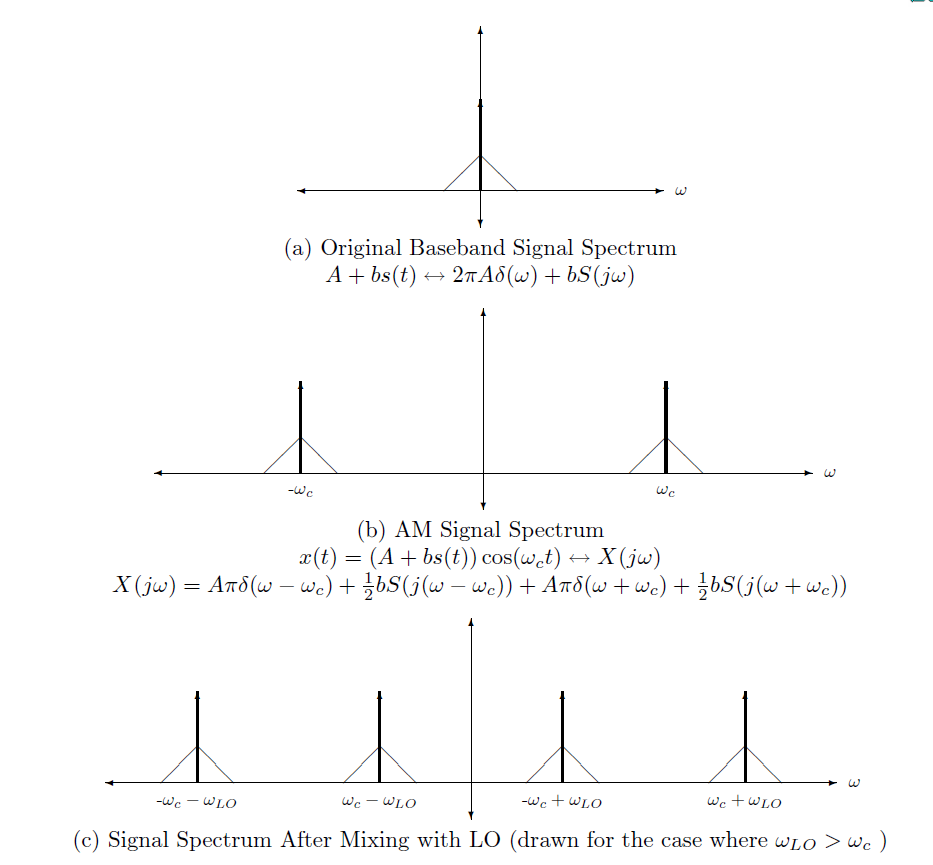
\includegraphics[scale=0.3]{P6.jpg}
\caption{Signal Spectrum (a) original signal, (b) signal at transmitter after AM modulation, (c) signal
at the output of the radio front-end mixer.}
\end{figure}
\subsection{IF Filter or How to Practically Select a Station and Demodulate a Signal}
The intermediate frequency (IF) filter shown in Fig. 2 is a bandpass filter centered at $f_{IF}$ (the IF
frequency). In the ideal case, the frequency response function of this filter would be that shown in Fig.7
below. Observe (see Fig. 6 (c)) that by choosing the LO frequency appropriately we can use the mixer to shift the frequency of the modulated signal so that the modulated signal passes through the IF filter
undistorted (assuming, of course, that the bandwidth of the IF filter exceeds the bandwidth of the message
signal). Either of two frequency choices are possible for the LO, namely (assuming $f_c>f_{IF})$
\begin{figure}[H]
\centering
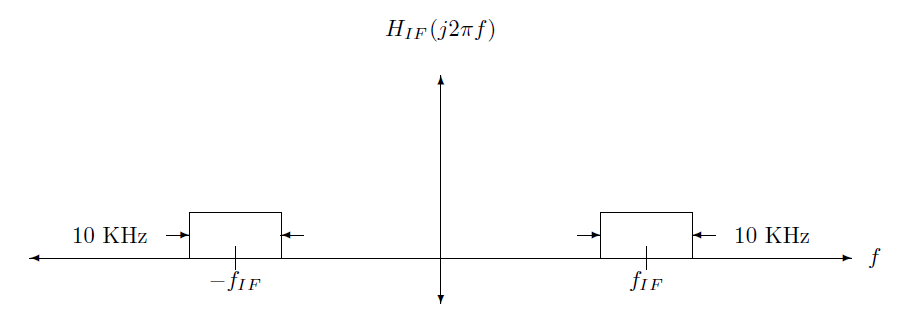
\includegraphics[scale=0.5]{P7.jpg}
\caption{Ideal IF Filter}
\end{figure}
\begin{equation}
\omega_{IF}=\omega_c-\omega_{LO}\rightarrow f_{LO}=f_c-f_{IF}
\end{equation}
or
\begin{equation}
\omega_{IF}=-\omega_c+\omega_{LO}\rightarrow f_{LO}=f_c+f_{IF}
\end{equation}
as indicated below in Fig. 8 and 9, respectively.
\begin{figure}[H]
\centering
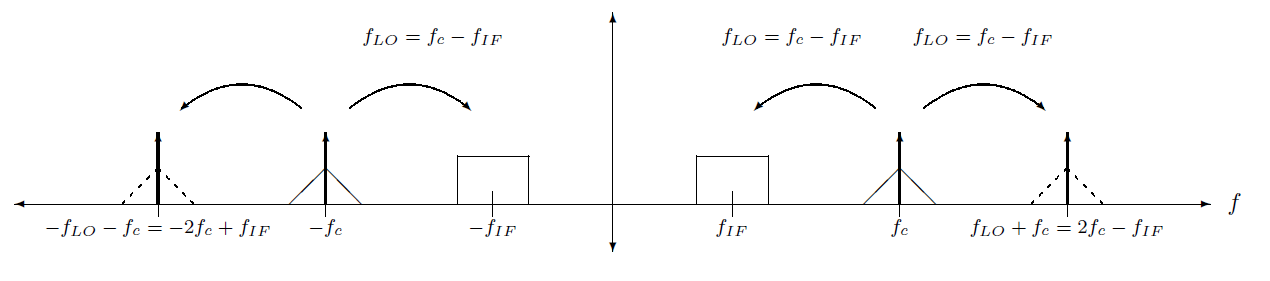
\includegraphics[scale=0.5]{P8.jpg}
\caption{Using LO to Mix into IF Band when $f_{LO}=f_c-f_{IF}$}
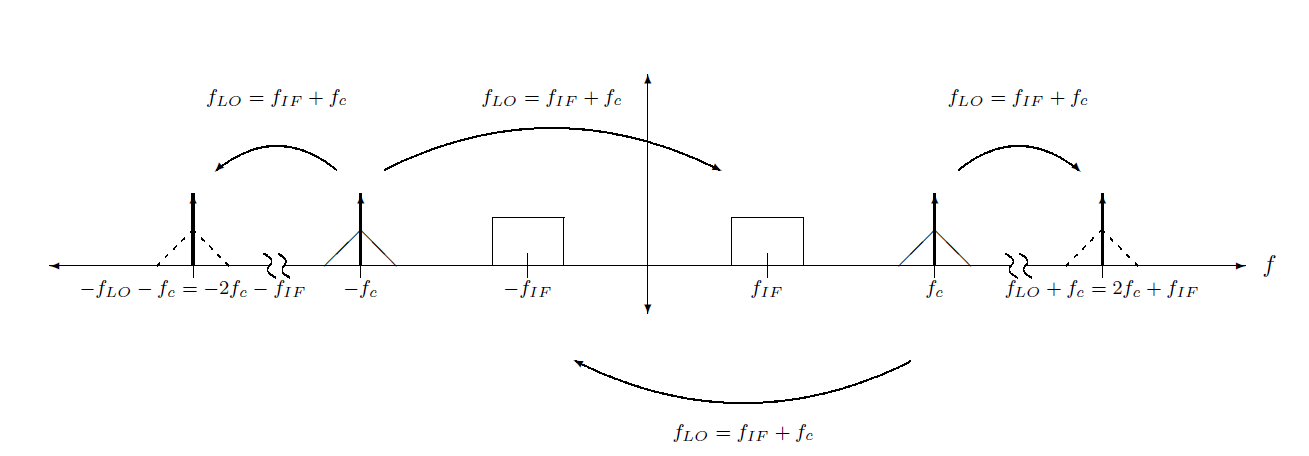
\includegraphics[scale=0.5]{P9.jpg}
\caption{Using LO to Mix into IF Band when $f_{LO}=f_c+f_{IF}$}
\end{figure}
In either case the output of the IF filter (up to a multiplicative constant) becomes
$$(A+bs(t))\cos(\omega_{IF}t+\phi-\theta)$$
Thus, if the output of the IF filter is fed into a properly designed envelope detector, the output
of the envelope detector will be $A+bs(t)$ (up to a multiplicative constant). Finally the constant term, $A$,
can be removed by placing a capacitor in series with the output of the envelope detector to
block the DC component, leaving just the information signal $s(t)$ (up to a multiplicative constant). Thus
our radio will have recovered the transmitted information signal, $s(t)$! A similar result is obtained when
$f_c<f_{IF}$. 
\subsection{A Simple Butterworth Filter Realization of the IF Filter}
We have seen that the IF filter should be a bandpass filter. Bandpass filters can take many different
forms. For example, a bandpass Butterworth filter of order N is characterized by the following (magnitude)
frequency response function.
\begin{equation}
|H(j\omega)|^2=\frac{H_o}{1+[2(\omega-\omega_0/\beta)]^{2N}}
\end{equation}
where the center frequency of the filter is $\omega_o$ rad/s, the peak gain is $H_o$ and the 3-dB bandwidth is 
$\beta$ rad/s. This filter approaches an ideal bandpass filter as N gets large, since for N large, the frequency
response function is nearly constant and equal to $H_o$ over the passband, $|\omega-\omega_o|<\beta$, and decreases rapidly
towards zero as one moves outside of the passband. Note that the 3-dB bandwidth alone does not indicate
the sharpness of the transition from passband to stop band. For the Butterworth filter, both the 3-dB
bandwidth and the filter order $N$ determine the filter performance.
\par In this lab, we will construct a very simple, op amp-based, IF filter. This filter does not have a particularly
sharp passband-to-stopband transition, but it is relatively simple to build and will be sufficient for our
application.
\par The frequency response function of our bandpass filter is given by
\begin{equation}
H(s)=H_o\frac{\beta s}{s^2+\beta s+\omega_o^2}
\end{equation}
where $s=j\omega$. Note that Eq. (23) can be rewritten as
\begin{equation}
H(j\omega)=H_o\frac{\beta j\omega_o}{(\omega_o+\omega)(\omega_o-\omega)+j\beta\omega}=H_o\frac{1}{\frac{\omega}{\omega_0}+j\frac{(\omega-\omega_0)}{\beta\omega_o/(\omega_o+\omega)}}
\end{equation}
For $\omega$ in the vicinity of $\omega_o$, Eq. (24) reduces to
\begin{equation}
H(j\omega)\approx H_o\frac{1}{\frac{\omega}{\omega_0}+j\frac{(\omega-\omega_0)}{\beta\omega_o/(\omega_o+\omega)}}=H_o\frac{1}{1+j\frac{(\omega-\omega_o)}{\beta/2}}
\end{equation}
It follows that the frequency response function in Eq. (25) achieves a maximum value of $H_o$ at a frequency
of $\omega_o$ rad/s with a 3-dB bandwidth equal to $\beta$ rad/s. Moreover, this result applies to our original frequency
response function as long as $\beta+\omega_o\approx\omega_o$, that is, when $\beta$ is a small fraction of $\omega_o$, which one typically writes as $\beta\ll\omega_o$.
\par The bottom line is that the bandpass filter in Eq. (24) achieves a maximum value of $H_o$ at a frequency
of $\omega_o$ rad/s with an approximate 3-dB bandwidth of
\begin{equation}
BW_{3dB}\approx\beta\text{vaild when } \beta\ll\omega_o
\end{equation}
\textbf{Image Frequencies:} This discussion is carried out for the case that the carrier frequency is greater than
the center frequency of the IF filter. Analyzing the other case is left to the reader.
\par By examining Fig. 9, one can see that when the LO frequency $f_{LO}$ is set equal to $f_c+f_{IF}$ , not only
does the signal centered at $f_c$ get mixed into the IF band, but so does any signal centered at
\begin{equation}
f_{imag}=f_{IF}+f_{LO}=f_c+2f_{IF}
\end{equation}
The frequency band centered at $f_{imag}$ is known as the image band. Using Eq. (27), we conclude that
\begin{equation}
f_{imag}-f_c=2f_{IF}\text{(valid when }f_{LO}=f{c}+f_{IF}\text{ \& }f_c>f_{IF}).
\end{equation}
Thus the separation between the carrier frequency of the desired station (i.e., the one you wish to receive)
and the center frequency of the image band (which also ends up in the passband of the IF filter after the
mixer) is equal to twice the IF frequency.
\par Then the separation between the carrier frequency of the desired station (i.e., the one you wish to receive)
and the center frequency of the image band is equal to
\begin{equation}
f_c-f_{imag}=\begin{cases}
2f_{IF}\qquad\qquad\quad f_c>2f_{IF}\\2(f_c-f_{IF}),\qquad f_c<2f_{IF}
\end{cases}
\text{(valid when }f_{LO}=f{c}+f_{IF}\text{ \& }f_c>f_{IF})
\end{equation}
\par We conclude that when the LO frequency is chosen to be the higher of the two possible choices, namely
$f_c+f_{IF}$, then the IF filter cannot separate two AM stations whose carrier frequencies differ by twice the
IF frequency, and according to Eq. (29), the separation between the desired and image stations may be
even less when the lower LO frequency is used. In either case, the RLC front-end (recall the antenna and
resonance tuning circuit) must sufficiently attenuate signals in the image band when tuned to the carrier
frequency of the desired station; otherwise, the image band will corrupt the demodulation of the desired
station. Consequently, the higher LO frequency is often chosen in order to simplify the design of the RLC
filter in the front-end. AM radios are designed so that both the LO frequency and the resonance frequency
of the RLC front-end are set together when a station is selected. The capacitor in the front-end RLC circuit
is adjusted so that the resonance frequency of this circuit is equal to the carrier frequency, $f_c$, of the station
that is to be received, while the LO frequency is set to one of the two frequencies $|f_c\pm f_{IF}|$.
\par The frequency selectivity (i.e., its $Q$) of a bandpass filter is a measure of its ability to attenuate signals
that do not lie near the center frequency of its passband, i.e., within a small fraction of the center frequency
of the passband. Consequently if the IF frequency is properly chosen, then the front-end RLC circuit does
not need to have much frequency selectivity in order to reject the image frequency because $\frac{f_c-f_{imag}}{f_c}=2\frac{f_{IF}}{f_{c}}$ when $f_{LO}=f_c+f_{IF}$. For example, if $f_{IF}$= 455 KHz, which is a common choice in commercial radios, then the desired and image frequencies are separated by 910 KHz and the front-end series RLC filter does not
require much frequency selectivity. The IF filter for the radio that you will build in this lab will be centered
at approximately 100 KHz.
\subsection{Why a Superheterodyne Receiver?}
\par A radio, like the one built in this lab experiment, which has an IF filter with a fixed center frequency and a
variable frequency LO (that can be used to shift the desired station into the IF band by mixing), is known
as a superheterodyne receiver. As mentioned earlier, the superheterodyne receiver was invented by Edwin
Armstrong in 1920 and is still widely used today.
\par It is natural to ask why we shouldn’t eliminate the LO, the mixer, and the fixed IF filter and replace these
elements by a single bandpass filter with a tunable center frequency. While such an approach is possible in
principle, it is difficult in practice to build tunable bandpass filters that have adequate frequency selectivity
and gain.
\par Perhaps an even better approach, then, would be to mix the frequency of the desired station down to
baseband (i.e., choose $f_{LO}=f_c$) and then simply low pass filter the output of the mixer. This approach,
however, may lead to a very weak signal, and one that will experience power fluctuations as the following
analysis indicates.
\par Consider the signal at the output of the mixer:
\begin{equation}
\begin{aligned}
(A+bs(t))\cos(\omega_c t+\phi)\cos(\omega_{LO}t+\theta)=\frac{1}{2}(A+bs(t))\cos((\omega_c+\omega_{LO})t+\phi+\theta)
\\+ \frac{1}{2}(A+bs(t))\cos((\omega_c-\omega_{LO})t+\phi-\theta)
\end{aligned}
\end{equation}
When $f_{LO}=f_c$, this signal becomes
\begin{equation}
(A+bs(t))\cos(\omega_c t+\phi)\cos(\omega_{LO}t+\theta)=\frac{1}{2}(A+bs(t))\cos(2\omega_c t+\phi+\theta)
+\frac{1}{2}(A+bs(t))\cos(\phi-\theta)
\end{equation}
The term at twice the carrier frequency will be strongly attenuated by the low-pass filter, leaving$\frac{1}{2}(A+bs(t))\cos(\phi-\theta)$ at the output. Note that for many values of $\phi-\theta$, for example, $\phi-\theta\approx\frac{\pi}{2}$ , the demodulated signal will be greatly diminished in strength. Indeed, for the case $\phi-\theta=\frac{\pi}{2}$, the signal strength is identically zero! It follows that when $|\cos(\phi-\theta)|\approx 0$, the presence of noise will significantly degrade the quality of reception. Furthermore, the relative phase difference between the carrier and the LO
would vary when the distance between the transmitter and the receiver changes, as in a moving car. Thus,
if the radio is moving, the demodulated signal strength will be time-varying (the radio would fade in and
out). Although radios can be built to track the relative phase and make LO adjustments to keep the relative
phase small (a method known as coherent reception), such radios are more expensive.
\par The use of envelope detection obviates the need to track the relative phase. There is, however, a price to
be paid for this simplicity. Envelope detection requires that a DC bias, $A$, be added to the signal before
modulation. This DC bias is chosen to ensure that the quantity $A+bs(t)$ always remains positive, otherwise
the message signal s(t) cannot be uniquely recovered from the envelope, $|A+bs(t)|$. The presence of the DC
bias term means that the transmitter must use additional power, since it needs to transmit both the signal
and the DC bias term. Because there are many fewer transmitters than receivers, it was decided in the early
days that it was better to burden the transmitter rather than the receiver with the extra cost. Given the
low cost and advanced state of electronics today, such a trade-off may no longer be favorable.
\section{Experimental Procedure}
\subsection{Modulated Sine Wave}
\begin{itemize}
\item Set the load of the function generator to be 50$\Omega$.
\item Use function generator to generate a modulated sine wave with baseband frequency 1kHz and modu-
lating frequency 100kHz.
\\The original signal should have 4V Vpp.
\\The carrier (modulating) signal should be sine wave as well.
\\The modulation depth should be 50% (modulation index 0.5).
\item Directly connect the generator to the ocsilloscope to verify your generated waveform. Store the images
with time division 200$\mu s$ and 20$\mu s$.
\item IThe mathematical formula of this waveform is given in the next part.
\end{itemize}
\subsection{Modulated Triangular Wave}
\begin{itemize}
\item Repeat last part, with the only difference that the original signal should have triangular shape.
\end{itemize}
\subsection{Envelop Detector}
\begin{itemize}
\item Assemble the circuit using $R=75K\Omega$ and $C=2.2nF$.
\item Use the envelope detector to "demodulate" the two signals in Part 1 and 2. Store your images still at
T = 200$\mu s$ and 20$\mu s$. In each image, be sure to display both CH1 (as input) and CH2 (as output).
\end{itemize}
\begin{figure}[H]
\centering
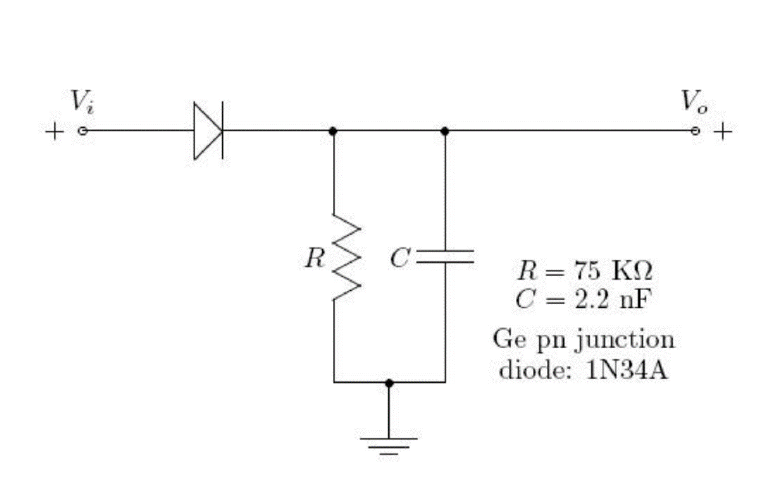
\includegraphics[scale=0.5]{P10.jpg}
\end{figure}
\subsection{Amplifier}
\begin{itemize}
\item Use the function generator to generate a 5kHz sine wave with 500 mV Vpp.
\item Assemble the circuit using $R1=15k\Omega,R_2=5.6k\Omega,R_3=82k\Omega$. and $C=220\mu F$ Capture both input
and output on the Ocsilloscope. Compare the measured gain of your amplier with the calculated value
\end{itemize}
\begin{figure}[H]
\centering
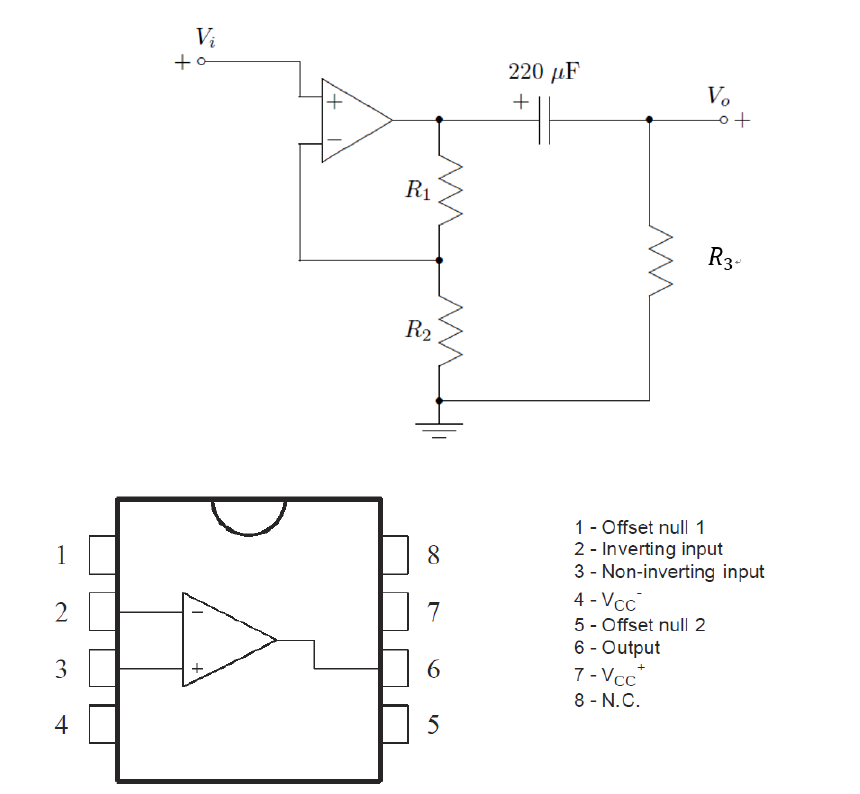
\includegraphics[scale=0.5]{P11.jpg}
\end{figure}
\section{Experimental Results}
\subsection{Modulated Sine Wave}
\begin{figure}[H]
\centering
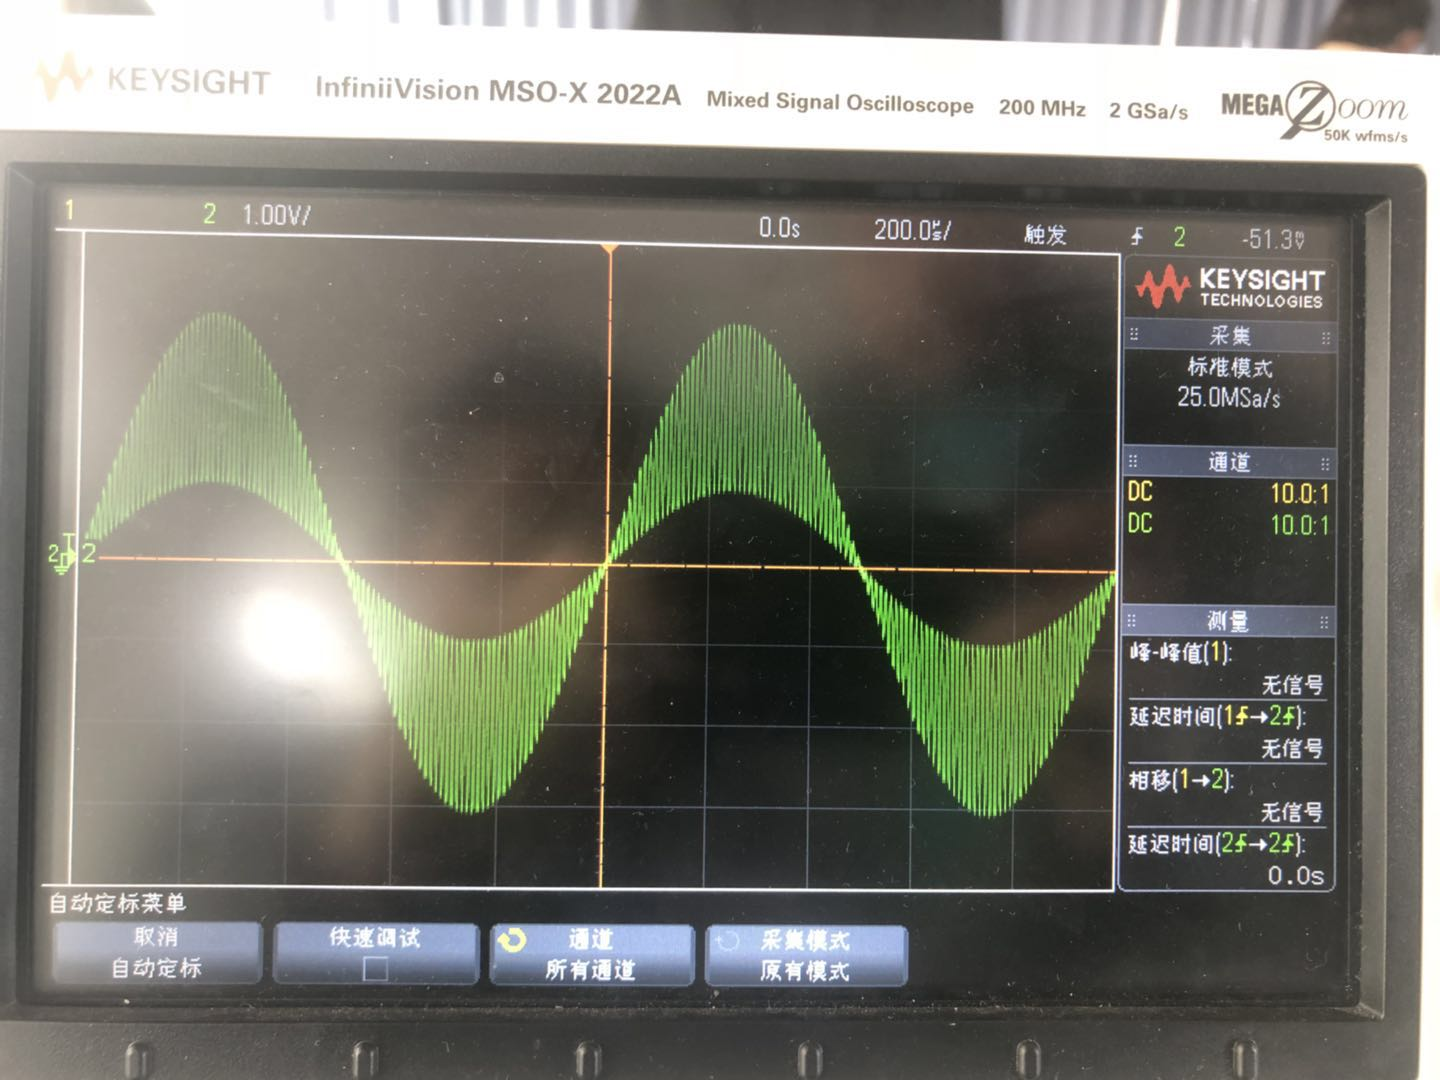
\includegraphics[scale=0.2]{P12.jpg}
\caption{Waveform with time division 200$\mu s$}
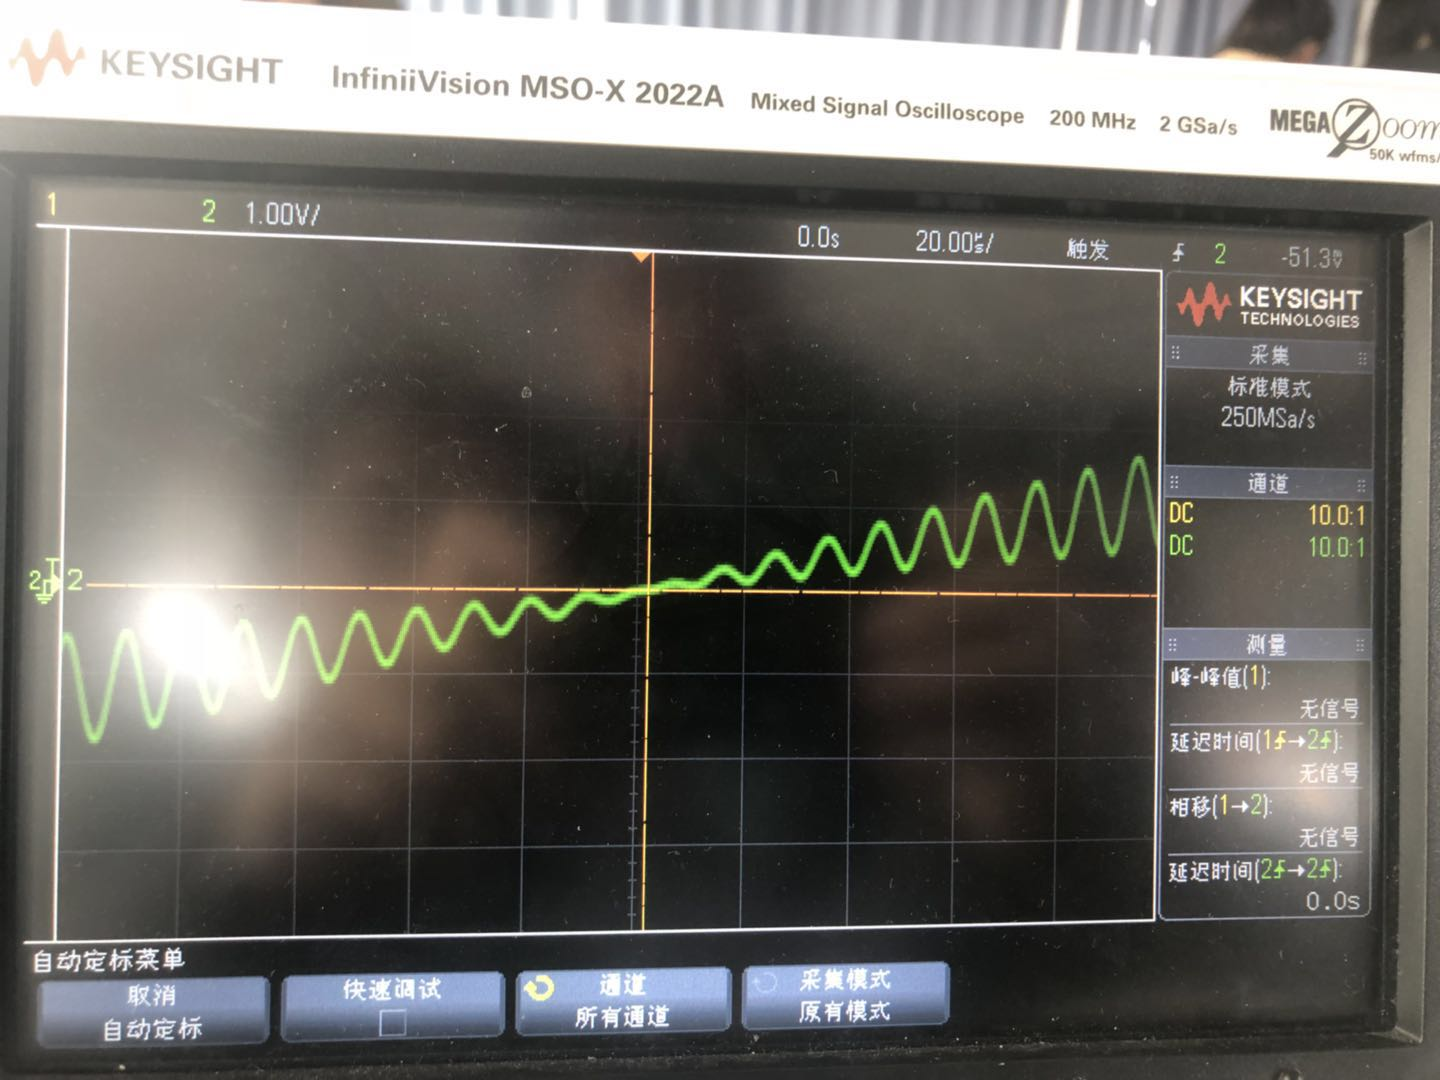
\includegraphics[scale=0.2]{P13.jpg}
\caption{Waveform with time division 20$\mu s$}
\end{figure}
According to the data from the manual, the formula is $$x(t)=(4+2\sin1000t)\cos(1000000t+\phi)$$
\subsection{Modulated Triangular Wave}
\begin{figure}[H]
\centering
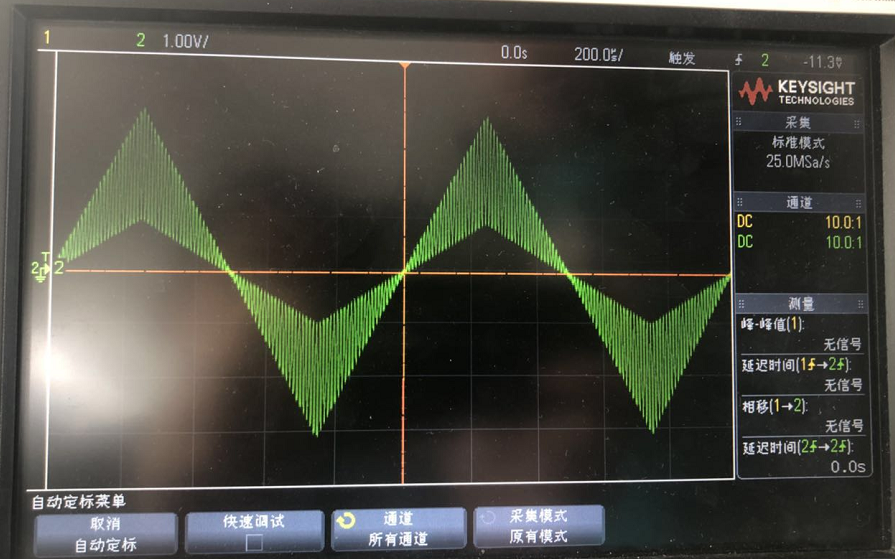
\includegraphics[scale=0.5]{P14.jpg}
\caption{Waveform with time division 200$\mu s$}
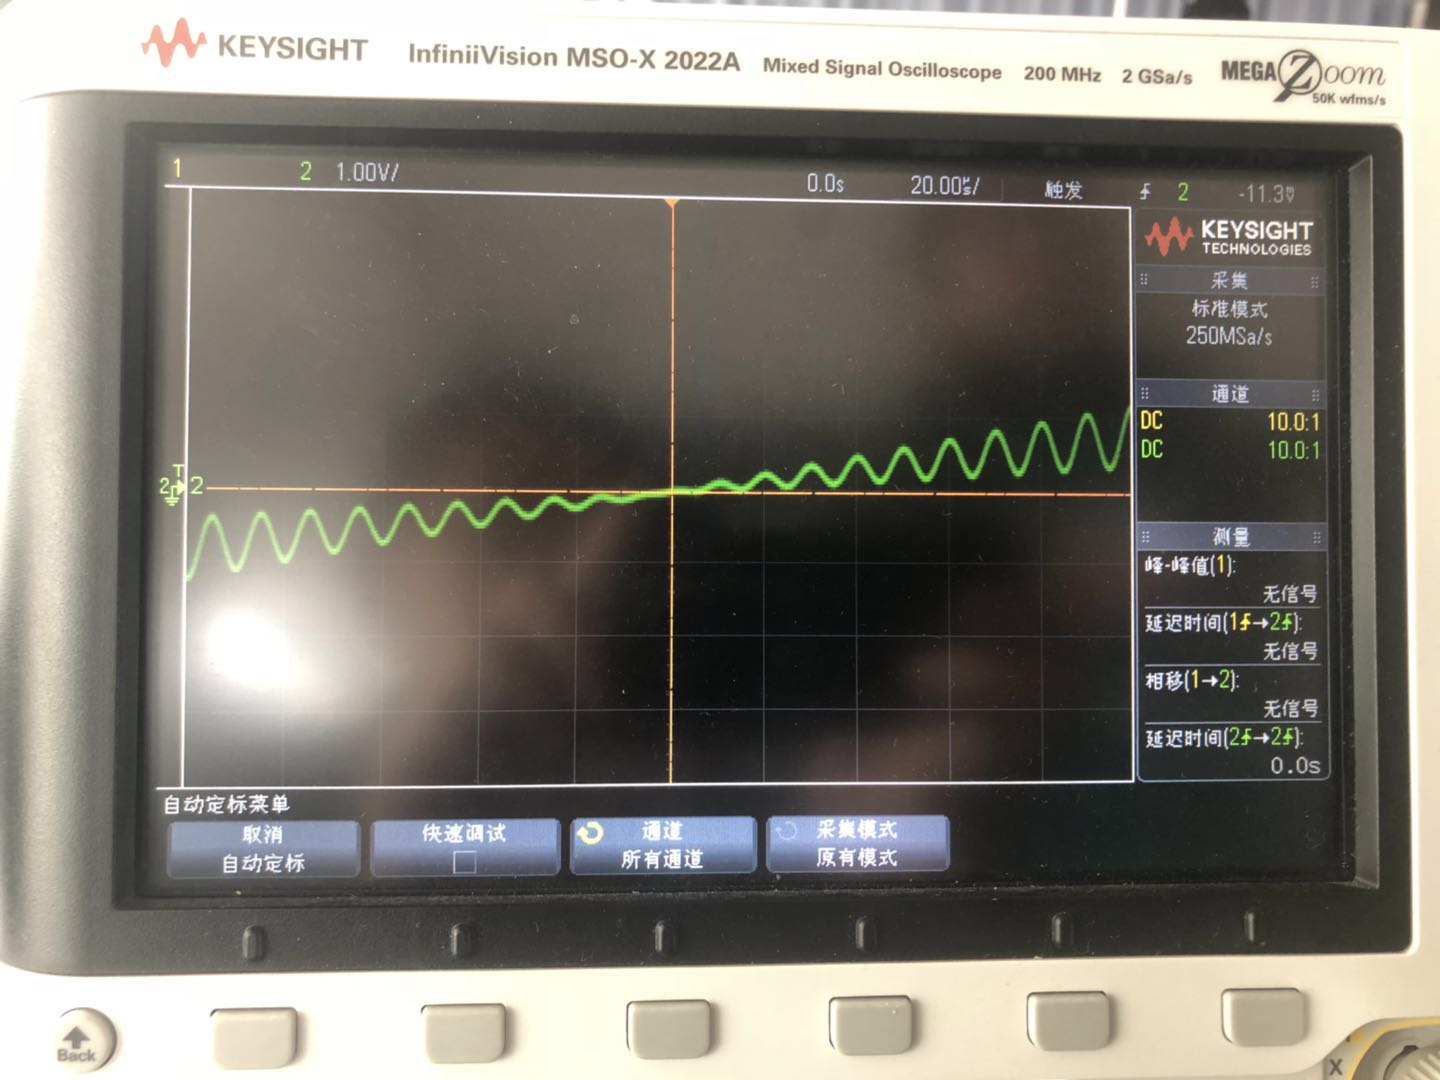
\includegraphics[scale=0.25]{P15.jpg}
\caption{Waveform with time division 20$\mu s$}
\end{figure}
\subsection{Envelop Detector}
\begin{figure}[H]
\centering
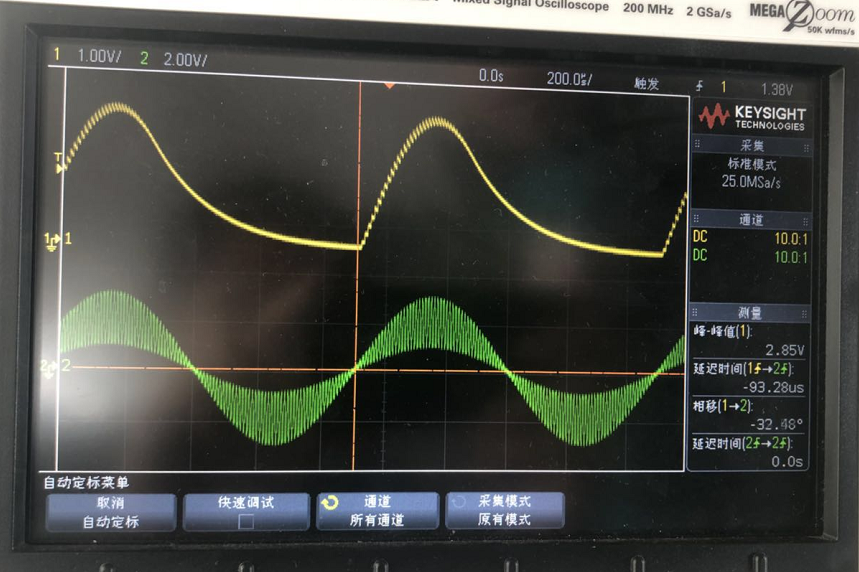
\includegraphics[scale=0.6]{P16.jpg}
\caption{Sine waveform with time division 200$\mu s$}
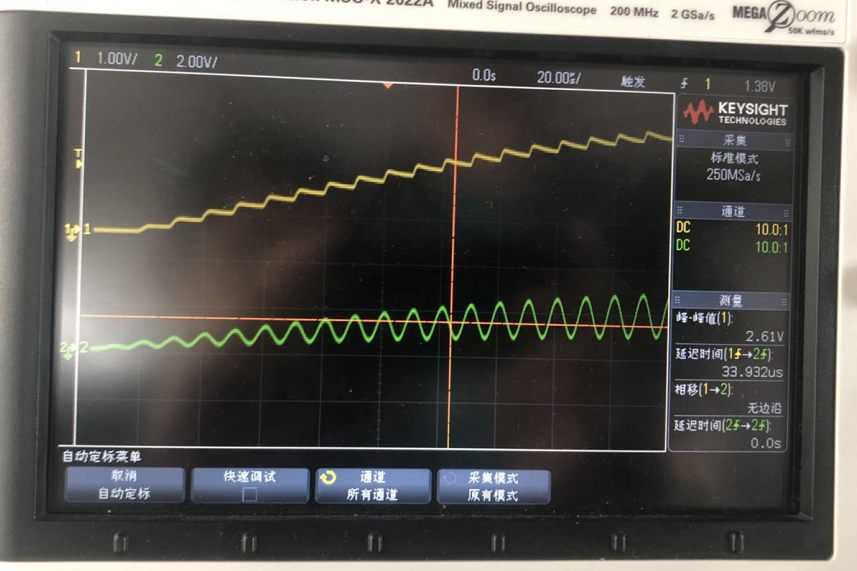
\includegraphics[scale=0.6]{P17.jpg}
\caption{Sine waveform with time division 20$\mu s$}
\end{figure}
\begin{figure}[H]
\centering
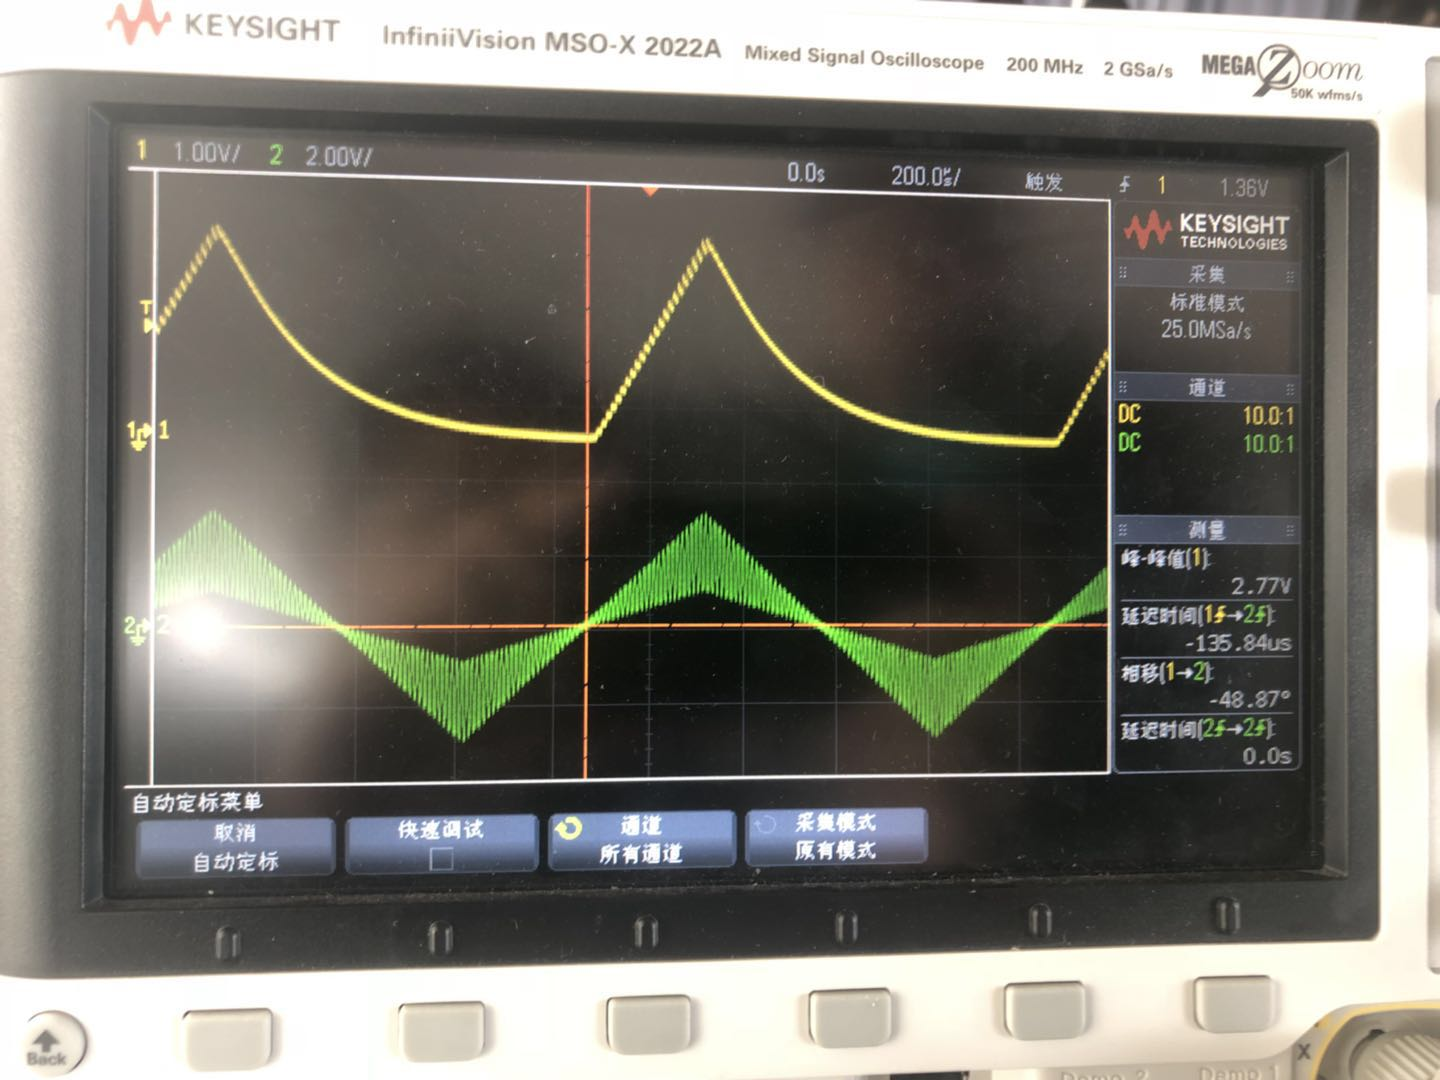
\includegraphics[scale=0.25]{P18.jpg}
\caption{Triangular waveform with time division 200$\mu s$}
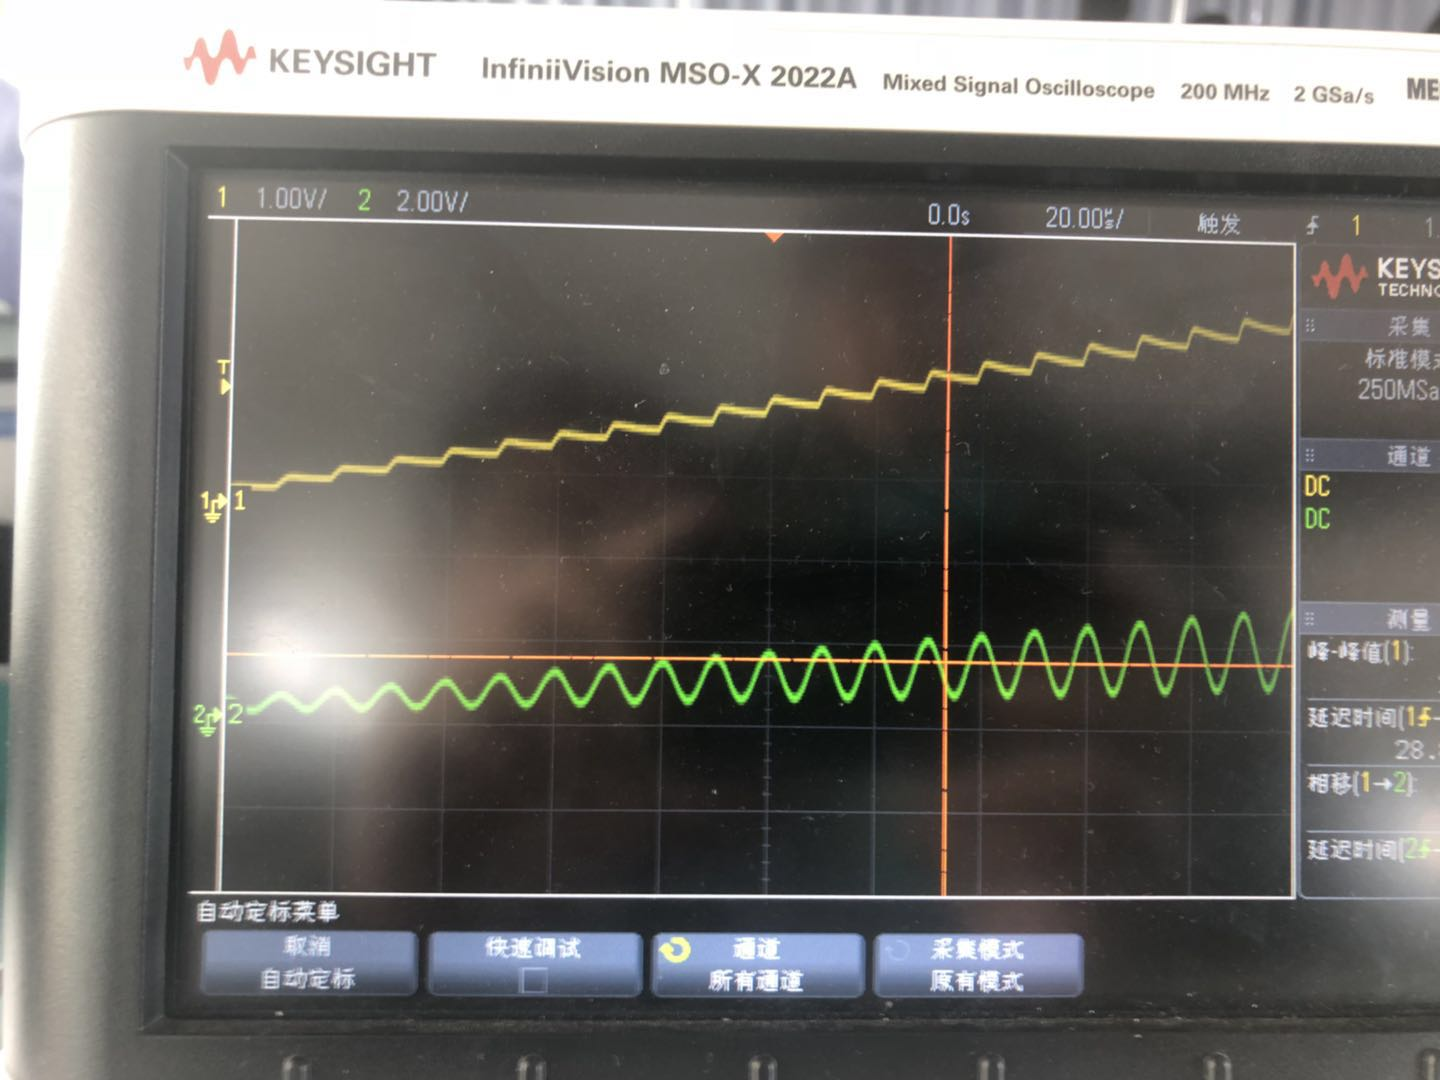
\includegraphics[scale=0.25]{P19.jpg}
\caption{Triangular waveform with time division 20$\mu s$}
\end{figure}
\subsection{Amplifer}
\begin{figure}[H]
\centering
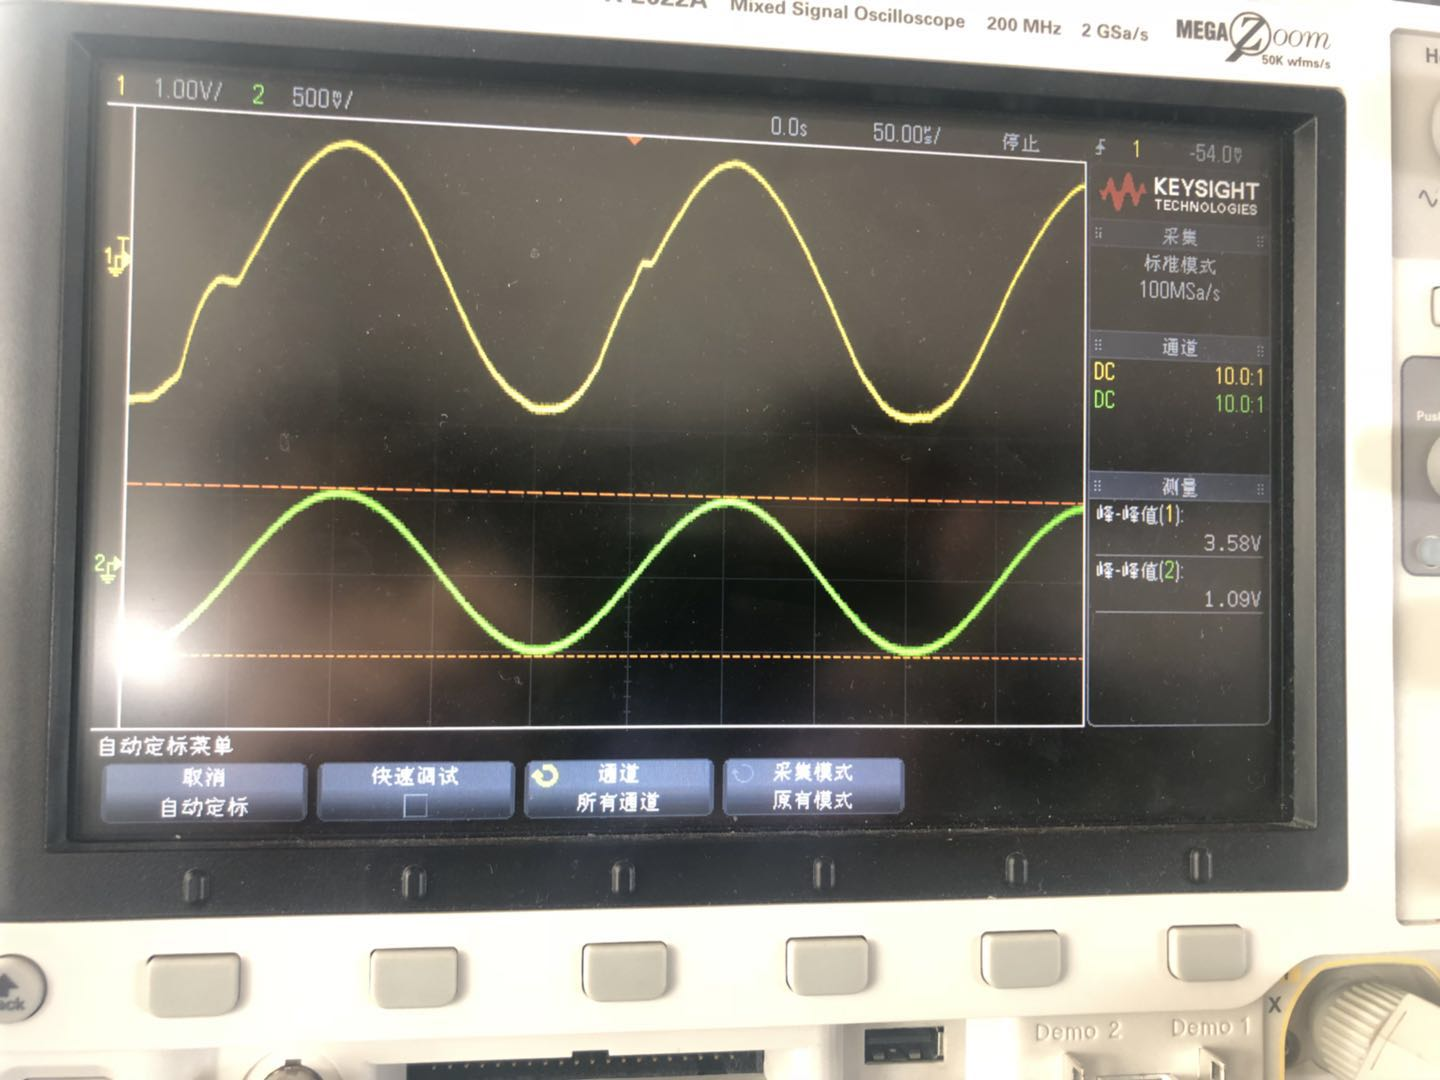
\includegraphics[scale=0.2]{P20.jpg}
\caption{Input and output figure for amplifier part}
\end{figure}
From the figure, we can read the Gain=$\frac{3.58}{1.09}\approx3.28$
\par According to the calculation:
$$\frac{R_1+R_2}{R+2}j\omega CV_i=\frac{1+j\omega CR_3}{R_3}V_i$$
the Gain=$\frac{V_o}{V_i}=|\frac{(R_1+R_2)R_3j\omega C}{(1+j\omega CR_3)R_2}|=3.68$, which is bigger than the measured one.
\section{Error Analysis and Discussion}
\subsection{Error Analysis}
In part 1, we modulate the Sine Wave and Triangular Wave, there is no error exist because we just created the input signal. And we record the form of them at T=200$\mu$s and 20$\mu$s.
\par In part 2, we let the signals we created in part 1 go through the Envelope Detector. 
And the ideal results should looks like this:
\begin{figure}[H]
\centering
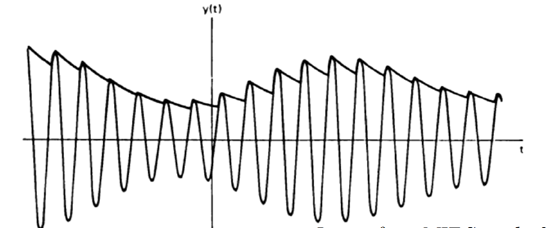
\includegraphics[scale=0.5]{P21.jpg}
\end{figure}
\par The output will approximately become the envelope and we obtain the “demodulated signal”. However, as we can see from Fig 14-17, though the input signal(the green one) changed abruptly, but the output signal(the yellow one) didn’t change as much as the input. That means the capacitor did prevent voltage changing abruptly.
\par But if we try to overlap the input and output signal, obviously, the output is quite close to the envelop the input, however, they cannot fully be identical, and that means there exist some error that influenced our results.
\par And in part 3, we let the input signal: 5kHz Sine Wave with 500mV Vpp go through our Amplifier. And we got that the Gain is about 3.28. But if we do the calculation:
$$\frac{R_1+R_2}{R+2}j\omega CV_i=\frac{1+j\omega CR_3}{R_3}V_i$$
so that the Gain=$\frac{V_o}{V_i}=|\frac{(R_1+R_2)R_3j\omega C}{(1+j\omega CR_3)R_2}|=3.68$
par So the absolute error is about 0.40, the relative error is 10.87\%. It’s not very large but also not small enough. We’ll discusses the causes of this error in Error Discussion part.
And also, the output signal was obviously not a pure Sine Wave, it’s also an error.
\subsection{Discussion of Error}
For the first error, I think it was unavoidable, because we know that only if the time constant of the RC combination is much longer than signal period, then the output will approximately become the envelope, in the experiment, we can figure out that the time constant of the RC combination is $\tau=RC=1.65\times 10^{-4}$,while the period of the input signal is $1\times 10^{-5}$, obviously it’s not “much longer”, so it’s reasonable if we found the output was not exactly the envelope of the input signal. Also, in the lab, we measured the value of $R$, it was not $75K\Omega$, it was actually $74765\Omega$, so the actual time constant was even lower.
\par For the second error, I think there were two reasons, and one was unavoidable, while another one is avoidable, or at least we can try to reduce it. The first reason is that, before we finished the circuit, we measured every resistors, and we found that the true values of these resistors are $81k\Omega$, $5.4k\Omega$ and $15.2k\Omega$, and also, when we do the calculation, we assumed the op amp is an ideal one, but in real life, there is no ideal op amp, this might be the reason why the output signal was not a pure Sine Wave.
\par So these are the errors that we cannot avoid.
\par And the second reason was that, actually when we got the figures, the output signal was shaking, and we need to use “Run Stop” button to stop this shaking and so we can read the data. So if we pressed the “Run Stop” button several times, and read different data, then calculated the average value, we might get a more accurate results.
\section{Conclusion}
\subsection{Prelab}
Before the lab, we learned some new knowledge and did some prelab assignments. We learned what is superherodyne AM receiver, and we know how it works. And what’s the meaning and working principles of Antenna and Tuned RLC Circuit. And how we can use Amplifier and Mixer to help us. We know how IF Filter works and why we need it. Also we took a review of many knowledges that we learned in VE215 last year, like the characteristic of op amp and diode.
\par And by doing the prelab assignment, we had a deeper understanding of the concepts like bandwidth, quality factor and so on. Also we learned how to use matlab to help us analyzing circuit.
\subsection{During Lab}
We used and became familar with the laboratory equipments, like the power supply, signal generator and digital oscilloscope. And by connecting the circuit ourselves, we had a deeper understanding of how Envelope detector and Amplifier works, and solving the problems appeared in the lab increased our analytical and strain capacity. 
\subsection{After Lab}
We comparing the ideal results with the figures and data we got from the lab, and find they are quite similar to each other, which confirmed the concepts we learned before. Also, after we analyzing the errors, we got to know how to improve our steps next time, and figured out the factors that may influence the results.
\par All in all, this lab is quite successful, we got the results we want, we reviewed the previous knowledge and learned new knowledge at the same time.
\end{document}